\section{二组分双液系}


\begin{frame}
    \frametitle{二组分体系}

    \large 对于二组分体系，根据相律，$C=2$时，$f=4-P$，$P$最小为1，所以自由度最多为3，即体系的状态最多可由三个独立变量来确定。这三个变量通常为温度、压力和组成($x$)，所以二组分体系的状态要用三个坐标的立体图形表示。

    \begin{minipage}{0.58\linewidth}
        为了简化讨论，通常固定其中一个变量，得到立体图形中的某一个截面图。这种平面图有三种：
        \begin{enumerate}
          \item $P-x$图
          \item $T-x$图
          \item $P-T$图
        \end{enumerate}
        在平面图上$f'=2$，同时共存相数最多为3。
    \end{minipage}\hfill
    \begin{minipage}{0.38\linewidth}
            \centering
            
\includegraphics[width=\linewidth]{3D-phase-diagram.png}
    \end{minipage}
\end{frame}


\begin{frame}
    \frametitle{理想完全互溶双液系}

    \large 两个纯液体组分可以按任意比例相互混合成均一液相的体系，称为完全互溶双液系。若混合溶液中任一组分在全部浓度范围内蒸气压与组成的关系都符合拉乌尔定律，则这样的双液系又称为理想完全互溶双液系。理想溶液即属于这一类体系。

    根据“相似相溶"的原则，一般说来，两种结构相似和极性相似的化合物（例如苯和甲苯、正己烷和正庚烷、邻二氯苯和对二氯苯或同位素的混合物、立体异构体的混合物等），大都能以任意的比例混合，并形成接近于理想的液态混合物。

\end{frame}


\begin{frame}
    \frametitle{定温下的$p$-$x$图}

    \begin{columns}[c]
        \column{6cm}
            \\~
            \\
            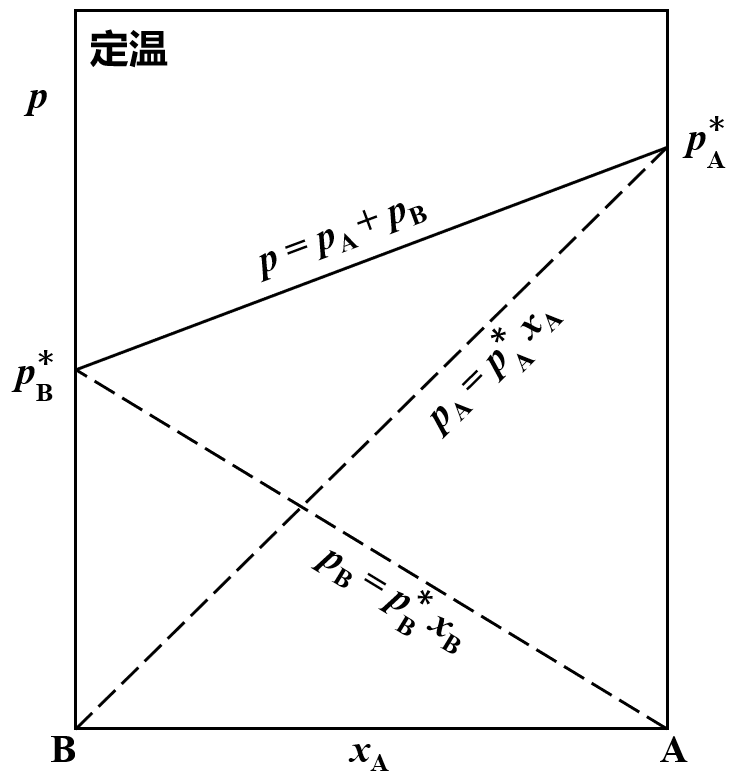
\includegraphics[width=6cm]{figs/p-x.png}
        \column{7.5cm}
            设组分A和B可形成理想溶液

            根据拉乌尔定律，有

            $p_\mathrm{A}=p_\mathrm{A}^* x_\mathrm{A}$

            $p_\mathrm{B}=p_\mathrm{B}^* x_\mathrm{B}=p_\mathrm{A}^*(1-x_\mathrm{A})$

            总蒸汽压

            $p = p_\mathrm{A}+p_\mathrm{B}= p_\mathrm{B}^* + (p_\mathrm{A}^*-p_\mathrm{B}^*)x_\mathrm{A}$

            根据此式，在定温下以$x_\mathrm{A}$为横坐标，$p$为纵坐标作$p$-$x$图为一直线。
    \end{columns}

\end{frame}


\begin{frame}
    \frametitle{定温下的$p$-$x$-$y$图}
    由于A、B二组分蒸汽压不同，则在某一温度下，当气液两相平衡共存时，气液两相的组成也不相同。
    \begin{columns}[c]
    \column{5.5cm}

            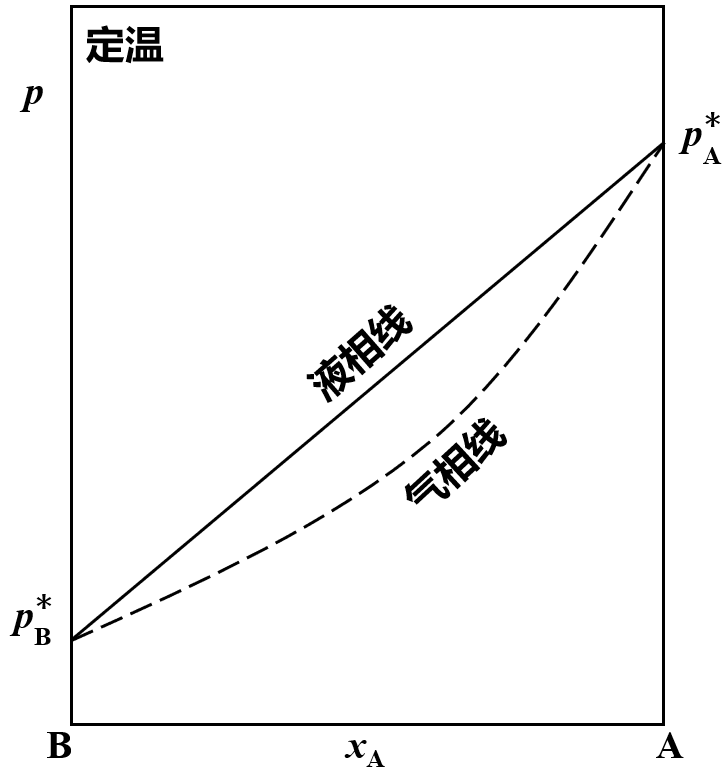
\includegraphics[width=5.5cm]{figs/p-x-y.png}
        \column{8.5cm}
            用y表示气相组成，根据分压定律
            {\footnotesize $$y_{\mathrm{A}}=\frac{p_{\mathrm{A}}}{p}=\frac{p_{\mathrm{A}}^{*} x_{\mathrm{A}}}{p_{\mathrm{B}}^{*}+\left(p_{\mathrm{A}}^{*}-p_{\mathrm{B}}^{*}\right) x_{\mathrm{A}}} \quad y_{\mathrm{B}}=\frac{p_{\mathrm{B}}^{*} x_{\mathrm{B}}}{p_{\mathrm{B}}^{*}+\left(p_{\mathrm{A}}^{*}-p_{\mathrm{B}}^{*}\right) x_{\mathrm{A}}}$$}
            设A为易挥发组分，$p_{\mathrm{A}}^{*}>p_{\mathrm{B}}^{*}$

            $\frac{y_{\mathrm{A}}}{y_{\mathrm{B}}}=\frac{p_{\mathrm{A}}^{*}}{p_{\mathrm{B}}^{*}} \cdot \frac{x_{\mathrm{A}}}{x_{\mathrm{B}}}>\frac{x_{\mathrm{A}}}{x_{\mathrm{B}}}$，$y_{\mathrm{A}}+y_{\mathrm{B}}=1$，$x_{\mathrm{A}}+x_{\mathrm{B}}=1$，故$y_{\mathrm{A}}>x_{\mathrm{A}}$

            易挥发组分在气相中的组成大于液相中组成；

            不易挥发组分在液相中的组成较大。

    \end{columns}
\end{frame}


\begin{frame}
    \frametitle{}
    \begin{block}{为什么饱和蒸气压越大越容易挥发？}
        当这种物质的蒸气的分压没有达到它的饱和蒸气压的时候，就会自发的有液态向气态转化的相变，也就是发生了蒸发现象或挥发现象。所以基本可以这样看---某温度下，物质的饱和蒸气压越大，那么就越容易挥发，直到空气中它的分压（或者说浓度）达到了饱和蒸汽压的数值，才达到平衡状态。
    \end{block}
\end{frame}


\begin{frame}
    \frametitle{定压下的$T$-$x$图}

    \begin{columns}[c]
        \column{4cm}    
            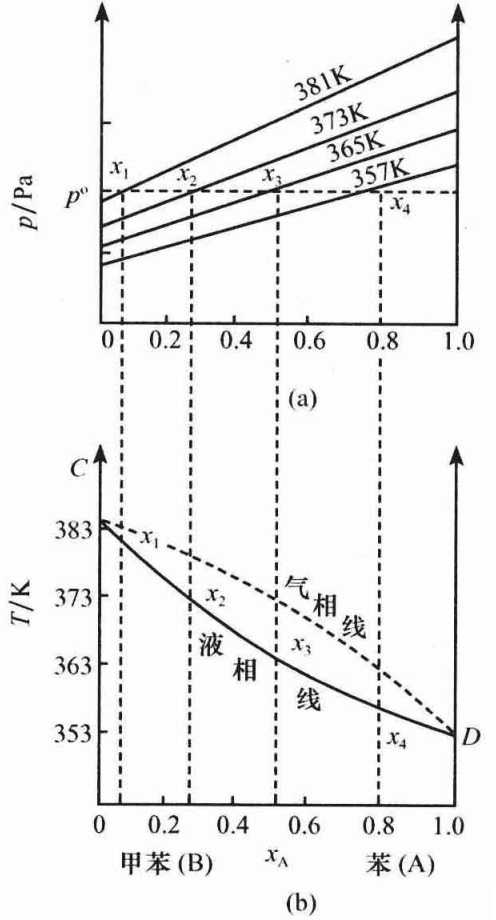
\includegraphics[width=3.98cm]{figs/p-x-2-T-x.png}
        \column{9.5cm}
        根据$p$-$x$图可给出定压下$T$-$x$图。以苯-甲苯双液系为例，首先在一系列不同温度下测定混合溶液总蒸气压与组成的关系，绘出一系列$p$-$x$线，如图（a）所示。在该图纵坐标为标准压力处作一水平线，与各$p$-$x$分别交于$x_1$、$x_2$、$x_3$、$\cdots$，所对应沸点分别为381.2K、373K、365.2K、$\cdots$。从沸点与组成的对应关系可得图（b）中的液相线，用同样的方法可从$p$-$x$图中的$p$-$y$线得到图（b）的气相线。

        \begin{enumerate}
          \item 在$T$-$x$图中，气相线在上，气相线以上为气态单相区
          \item 液相线以下为液态单相区
          \item 中间月牙部分为气、液两相共存区
        \end{enumerate}
    \end{columns}
\end{frame}


\begin{frame}
    \frametitle{物系点与相点}

    相图中表示体系总组成状态的点称物系点；表示各相组成和状态的点称为相点。
    \medskip

        \begin{minipage}{0.6\linewidth}
            \begin{enumerate}
              \item 当组成为$x_\mathrm{A}$的体系处于温度$T_1$时，此时体系只有一个气相存在，$S$点既表示体系总组成又表示气相组成，既为物系点又为相点。
              \item 当体系降温至$T_2$时，物系点沿垂线下移到$C$点，此时气、液两相平衡共存，过$C$点作一与横轴平行的直线，分别交气相线、液相线于两点，即表示体系气相组成的气相点$E$和体系液相组成的液相点$D$，可见二相平衡共存区内物系点与相点分离。
              \item 当体系继续降温至$T_3$时物系点为$P$，此时为液态单相区，物系点即为相点。
            \end{enumerate}
        \end{minipage}\hfill
        \begin{minipage}{0.38\linewidth}
            \begin{figure}[htpb]
                \centering
                
\includegraphics[width=\linewidth]{level-rule.png}
            \end{figure}
        \end{minipage}
\end{frame}


\begin{frame}
    \frametitle{杠杆规则}

    \begin{columns}[c]
        \column{7.5cm} 
            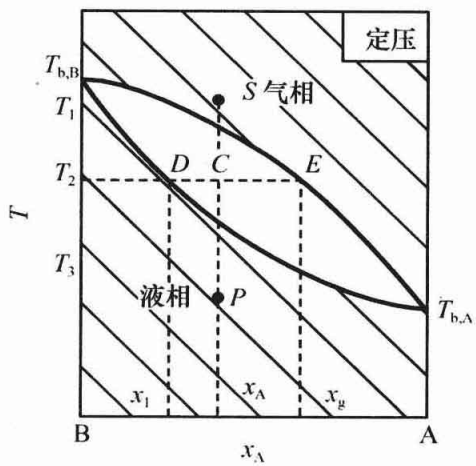
\includegraphics[width=7.5cm]{figs/level-rule.png}
        \column{6cm}
            当体系处在物系点$C$时，总组成为$x_\mathrm{A}$，总物质的量为$n$ mol；
            
            气相组成$x_\mathrm{g}$，共有$n_\mathrm{g}$ mol物质；

            液相组成$x_\mathrm{l}$，共有$n_\mathrm{l}$ mol物质。
            $$\begin{aligned}
            n&=n_{1}+n_{\mathrm{g}} \\
            n x_{\mathrm{A}}&=n_{1} x_{1}+n_{\mathrm{g}} x_{\mathrm{g}} \\
            n_{1}(x_{\mathrm{A}}-x_{1})&=n_{\mathrm{g}}(x_{\mathrm{g}}-x_{\mathrm{A}})
            \end{aligned}$$
            则
            $$\frac{n_{1}}{n_{\mathrm{g}}}=\frac{x_{\mathrm{g}}-x_{\mathrm{A}}}{x_{\mathrm{A}}-x_{1}}=\frac{\overline{C E}}{\overline{D C}}$$
    \end{columns}    
\end{frame}


\begin{frame}[t]
    \frametitle{}

    \begin{example}
        由A、B组成的理想互溶双液系，在某温度下气液两相平衡时$n$(g)=3mol，$n$(l)=5mol，此时液相的组成$x_\mathrm{B}$(l)=0.2，气相组成$x_\mathrm{B}$(g)=0.7，求体系的组成$x_\mathrm{B}$。
    \end{example}\pause

    \begin{columns}
        \column{6.75cm}
            $$n=n(\mathrm{g})+n(\mathrm{l})=8\mathrm{mol}$$
            $$8 x_{\mathrm{B}} =5\times 0.2 +3 \times 0.7$$
            $$x_{\mathrm{B}}=0.39$$
        \columnseprule=1pt
        \column{6.75cm}
            $$5(x_{\mathrm{B}}-0.2)=3(x_{\mathrm{B}}-0.7)$$
            $$x_{\mathrm{B}}=0.39$$
    \end{columns}
\end{frame}


\begin{frame}
    \frametitle{精馏原理}

    精馏是利用混合物中各组分挥发度不同而将各组分加以分离的一种分离过程，常用的设备是精馏塔。将气相部分冷凝，可使气相组成沿气相线下降，最后得到易挥发的低沸点组分；将液相部分汽化，液相组成沿液相线上升，最后得到难挥发的高沸点组分。

\begin{figure}[htpb]
    \centering
    \setcounter{subfigure}{0}
    \subfloat{
\includegraphics[height=4.5cm]{精馏塔}}\qquad
    \subfloat{
\includegraphics[height=4.5cm]{rectification}}
\end{figure}

\end{frame}


\begin{frame}
    \frametitle{非理想完全互溶双液系}

    \large 实际上经常遇到的完全互溶双液系绝大多数是非理想混合物，它们不能在全部浓度范围内遵守拉乌尔定律，称为非理想完全互溶双液系。
    
    根据其与理想溶液相比所产生的偏差大小，大致可分三类。

    \begin{itemize}
        \item[\bullet] 正负偏差都不大
        \item[\bullet] 正偏差很大
        \item[\bullet] 负偏差很大
    \end{itemize}

\end{frame}


\begin{frame}
    \frametitle{正负偏差都不是很大的体系}

    此类体系有\ce{CH3OH}-\ce{H2O}，\ce{C6H6}-\ce{CH3COCH3}，\ce{CH3Cl}-\ce{C2H5OC2H5}，\ce{CCl4}-\ce{C6H6}等。
    
    在此类相图中，气、液相线都不是直线。

        \begin{figure}[htpb]
            \centering
            \setcounter{subfigure}{0}
            \subfloat{
\includegraphics[height=4cm]{正偏差}}\hfill
            \subfloat{
\includegraphics[height=4cm]{负偏差}}\hfill
            \subfloat{
\includegraphics[height=4cm]{3.7a}}
        \end{figure}

\end{frame}


\begin{frame}
    \frametitle{正偏差很大的体系}

    此类体系有\ce{C2H5OH-H2O}，\ce{C2H5OH-C6H6}，\ce{CH3OH-C6H6}等。

    由于$p_\mathrm{A}$、$p_\mathrm{B}$偏离拉乌尔定律都很大，因此在$p-x$图上产生最高点，相应的在$T-x$图上出现最低点，此时对应的体系称为共沸溶液或共沸混合物。溶液的蒸气压恒大于两个纯组分的蒸气压。溶液的沸点恒低于两个纯组分的沸点。

    $$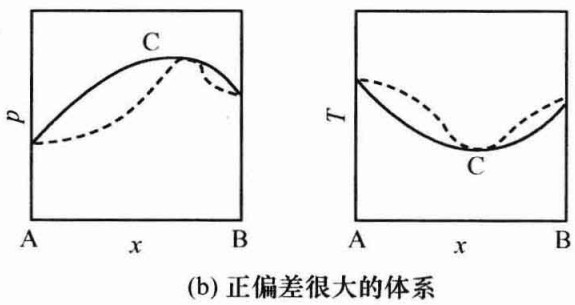
\includegraphics[height=4cm]{figs/3.7b.png}$$

\end{frame}


\begin{frame}
    \frametitle{负偏差很大的体系}

    此类体系有\ce{HCl-H2O}，\ce{HNO3-H2O}等。

    在$p-x$图上产生最低点，在$T-x$图上产生最高点。
    
    溶液的蒸气压恒低于纯组分的蒸气压，溶液的沸点恒高于任一组分的沸点。

    $$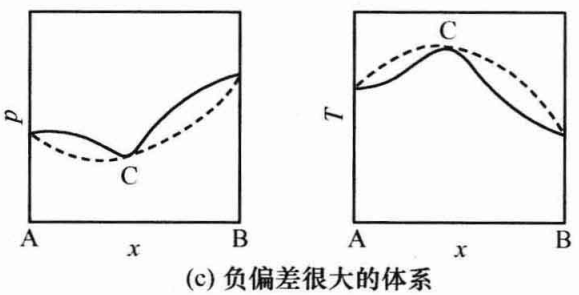
\includegraphics[height=4cm]{figs/3.7c.png}$$

\end{frame}


\begin{frame}
    \frametitle{非理想完全互溶双液系气-液平衡相图}

    \begin{columns}[c]
        \column{4.8cm}
            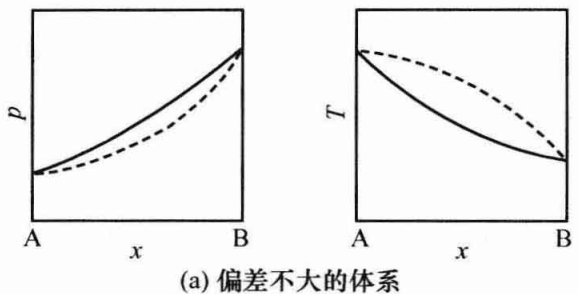
\includegraphics[width=4.7cm]{figs/3.7a.png}
            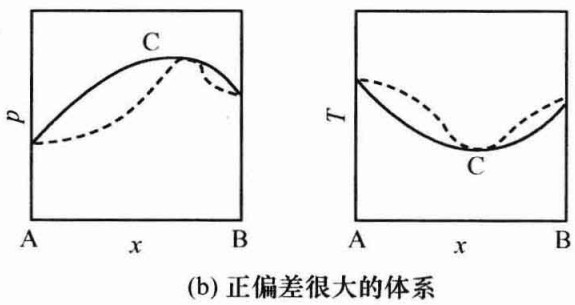
\includegraphics[width=4.7cm]{figs/3.7b.png}
            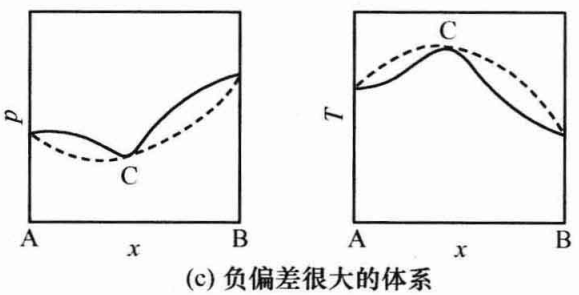
\includegraphics[width=4.7cm]{figs/3.7c.png}
        \column{8.7cm}
            (b)、(c)类相图可认为是由两个完全互溶双液系相图(a)组合成的。

            当体系的物系点为最高点(或最低点)$C$时，气、液两相组成相同，即$x_\mathrm{l}=x_\mathrm{g}$，加热至沸腾，沸点始终不变，此点$f^*=0$称为恒沸点(有最高、最低之分)。该组成的混合物称为恒沸混合物，它的组成随压力的改变而发生变化。

            由于恒沸点存在，对于后两类体系，无法通过蒸馏同时得到纯组分$A$和$B$，只能得到纯$A$和组成为$C$的混合物或得到纯$B$和组成为$C$的混合物。
    \end{columns}

\end{frame}